% Arbeitsblatt 2 – Questions on the text: your scaffold (nach Skills S3.2)
% Übersetzen: xelatex ab-2-questions-on-the-text.tex (zweimal)
% Lösungsfassung: ab-2-questions-on-the-text-lsg.tex
% ============================================================
% ab-vorlage.tex – gemeinsame Vorlage der Arbeitsblätter
% englisch/13/questions-on-the-text/arbeitsblaetter/
% Übersetzen mit:  xelatex <datei>.tex   (zweimal, wegen Seitenzahlen)
% Lösungsfassung:  Einzeiler-Datei <datei>-lsg.tex mit
%                  \def\mitloesung{}\input{<datei>}
% Schriften: Carlito (Fließtext), Poppins (Überschriften), TeX Gyre Pagella (Texte)
% ============================================================
\documentclass[10pt,a4paper]{article}
\usepackage[a4paper,top=12mm,bottom=13mm,left=14mm,right=14mm,headsep=4mm,headheight=12pt,footskip=7mm]{geometry}
\usepackage{fontspec}
\setmainfont{Carlito}
\newfontfamily\headfont{Poppins}[UprightFont=* Medium, BoldFont=* Medium]
\newfontfamily\headlight{Poppins Light}
\newfontfamily\lorafont{TeX Gyre Pagella}
\usepackage{xcolor}
\definecolor{prim}{HTML}{2563EB}
\definecolor{primdark}{HTML}{1E3A8A}
\definecolor{sec}{HTML}{7C3AED}
\definecolor{primtint}{HTML}{EFF6FF}
\definecolor{sectint}{HTML}{F5F3FF}
\definecolor{ink}{HTML}{1E293B}
\definecolor{muted}{HTML}{64748B}
\definecolor{rule}{HTML}{CBD5E1}
\definecolor{good}{HTML}{059669}
\definecolor{goodtint}{HTML}{ECFDF5}
\definecolor{warn}{HTML}{B45309}
\definecolor{warntint}{HTML}{FFFBEB}
\definecolor{bad}{HTML}{B91C1C}
\definecolor{badtint}{HTML}{FEF2F2}
\color{ink}
\usepackage[most]{tcolorbox}
\usepackage{tikz}
\usetikzlibrary{positioning,calc,arrows.meta,shapes.misc}
\usepackage{enumitem}
\setlist{nosep,leftmargin=1.1em,topsep=1pt}
\setlist[itemize]{label=\textcolor{prim}{\small\textbullet}}
\usepackage{tabularx,array,booktabs,colortbl}
\usepackage{multicol}
\usepackage{fancyhdr}
\usepackage{lastpage}
\usepackage{amssymb}
\usepackage{microtype}
\setlength{\parindent}{0pt}
\setlength{\parskip}{0pt}
\linespread{1.02}

% ---------- Kopf- und Fußzeile ----------
\newcommand{\wskopf}{English · Q13 · Science and Technology}
\pagestyle{fancy}
\fancyhf{}
\renewcommand{\headrulewidth}{0pt}
\fancyhead[L]{\footnotesize\headlight\textcolor{muted}{\wskopf}}
\fancyhead[R]{\footnotesize\headlight\textcolor{muted}{Name: \rule{38mm}{0.3pt}\quad Date: \rule{18mm}{0.3pt}}}
\fancyfoot[L]{\scriptsize\textcolor{muted}{edu-mrh.de/englisch/13/questions-on-the-text}}
\fancyfoot[R]{\scriptsize\textcolor{muted}{\thepage\,/\,\pageref*{LastPage}}}

% ---------- Titel ----------
% \wstitel{Kürzel}{Titel}{Untertitel}
\newcommand{\wstitel}[3]{%
  \begin{tcolorbox}[enhanced,colback=prim,colframe=prim,arc=2mm,boxrule=0pt,
     left=4mm,right=4mm,top=2.2mm,bottom=2.2mm,
     interior style={left color=primdark,right color=sec}]
    \color{white}{\headlight\footnotesize #1}\\[0.3mm]
    {\headfont\LARGE #2}\\[0.6mm]
    {\small #3}
  \end{tcolorbox}\vspace{1mm}}

% ---------- Boxen ----------
% \begin{wsbox}{Nummer}{Überschrift} ... \end{wsbox}
\newtcolorbox{wsbox}[3][]{enhanced,breakable,colback=white,colframe=rule,boxrule=0.5pt,arc=1.5mm,
  left=2.5mm,right=2.5mm,top=1.3mm,bottom=1.3mm,
  title={\headfont\normalsize\textcolor{white}{\colorbox{prim}{\,#2\,}}\;\textcolor{ink}{#3}},
  coltitle=ink,colbacktitle=white,attach title to upper={\par\vspace{0.6mm}},before skip=1.4mm,after skip=1.4mm,#1}
\newtcolorbox{tintbox}[1][]{enhanced,colback=primtint,colframe=primtint,boxrule=0pt,arc=1.2mm,
  left=2mm,right=2mm,top=1.2mm,bottom=1.2mm,#1}
\newtcolorbox{secbox}[1][]{enhanced,colback=sectint,colframe=sectint,boxrule=0pt,arc=1.2mm,
  left=2mm,right=2mm,top=1.2mm,bottom=1.2mm,#1}
\newtcolorbox{goodbox}[1][]{enhanced,colback=goodtint,colframe=goodtint,boxrule=0pt,arc=1.2mm,
  left=2mm,right=2mm,top=1.2mm,bottom=1.2mm,#1}
\newtcolorbox{warnbox}[1][]{enhanced,colback=warntint,colframe=warntint,boxrule=0pt,arc=1.2mm,
  left=2mm,right=2mm,top=1.2mm,bottom=1.2mm,#1}
\newtcolorbox{badbox}[1][]{enhanced,colback=badtint,colframe=badtint,boxrule=0pt,arc=1.2mm,
  left=2mm,right=2mm,top=1.2mm,bottom=1.2mm,#1}

\newcommand{\kl}[1]{{\headfont\small\textcolor{prim}{#1}}}      % kleine Zwischenüberschrift
\newcommand{\klsec}[1]{{\headfont\small\textcolor{sec}{#1}}}
\newcommand{\plus}{\textcolor{good}{\textbf{+}}\ }
\newcommand{\minus}{\textcolor{bad}{\textbf{–}}\ }
\newcommand{\pfeil}{\textcolor{prim}{$\rightarrow$}\ }
\newcommand{\linie}[1][\linewidth]{\rule{#1}{0.3pt}}
% ---------- Lösungsschalter ----------
% \lsg[Breite]{Text}        Lücke mit Unterstrich; Lösung erscheint nur mit \mitloesung
% \lsglinien{n}{Text}       n Schreiblinien; Lösung wird auf die Linien geschrieben
% Beide reservieren in beiden Fassungen exakt denselben Platz.
\newif\ifloesung
\ifdefined\mitloesung \loesungtrue \else \loesungfalse \fi
\newcommand{\lsgstil}{\color{sec}\itshape}
\newcommand{\lsg}[2][30mm]{%
  \makebox[#1][l]{\rlap{\raisebox{-0.8mm}{\textcolor{rule}{\rule{#1}{0.4pt}}}}%
  \ifloesung{\lsgstil\small #2}\fi}}
\newlength{\lsgzeile}\setlength{\lsgzeile}{7mm}
\newcommand{\lsglinien}[2]{%
  \par\noindent
  \begin{tikzpicture}[x=1mm,y=1mm]
    \pgfmathsetmacro{\hoehe}{#1*7}
    \path[use as bounding box] (0,0.5) rectangle (\linewidth,-\hoehe);
    \foreach \i in {1,...,#1} {\draw[rule,line width=0.4pt] (0,-\i*7) -- (\linewidth,-\i*7);}
    \ifloesung
      \node[anchor=north west,inner sep=0pt,text width=\linewidth,align=left,
            font=\lsgstil\small] at (0,-3.3) {\setlength{\baselineskip}{\lsgzeile}#2\par};
    \fi
  \end{tikzpicture}\par}
\newcommand{\schreiblinien}[1]{\lsglinien{#1}{}}


\begin{document}
\fontsize{9.4}{10.9}\selectfont

\wstitel{Worksheet 2 · Skills S3.2 · Analysing non-fictional texts}{Questions on the text — your scaffold}%
{One routine for every factual text: in class, at home and in the exam. Fill in the gaps while we work on the Baxter text (book p.\,230).}

% ------------------------------------------------------------------ 0
\begin{wsbox}{0}{Know the task — the operator tells you what to do}
\renewcommand{\arraystretch}{1.12}
\begin{tabularx}{\linewidth}{@{}>{\raggedright\arraybackslash}p{30mm}>{\raggedright\arraybackslash}p{42mm}>{\raggedright\arraybackslash}X@{}}
\kl{Level} & \kl{Typical operators} & \kl{You … / you don't …}\\\arrayrulecolor{rule}\midrule
\textbf{I Comprehension}\newline \textcolor{muted}{\emph{What does the text say?}} & describe, outline, sum up, state, point out & give the relevant content in your \emph{own words} with line references · no stylistic analysis, no opinion\\
\textbf{II Analysis}\newline \textcolor{muted}{\emph{How does it say it — and why?}} & analyse, examine, explain, compare, characterise & show how structure, language, style and tone \emph{support the message} — with quotes · no retelling, no opinion\\
\textbf{III Evaluation}\newline \textcolor{muted}{\emph{What do you think — and why?}} & comment, discuss, assess, evaluate & take a justified position, separate from the facts, with arguments and examples\\
\end{tabularx}
\end{wsbox}

% ------------------------------------------------------------------ 1
\begin{wsbox}{1}{Step 1 · Preparation}
\begin{minipage}[t]{0.40\linewidth}\vspace{0pt}
\begin{enumerate}[label=\textcolor{prim}{\textbf{\alph*}},leftmargin=1.2em]
\item \textbf{Read the questions first}, mark the operators.
\item \textbf{Skim} the text: topic and main arguments.
\item \textbf{Find out the purpose}: text type and its typical features (S3.1), source, author, date, target group.
\item \textbf{Understand}: read again, mark key words, sum up each section in the margin (3–6 words).
\end{enumerate}
\vspace{1mm}
{\footnotesize\textcolor{muted}{Marking idea: number the sections \textcircled{\scriptsize 1} \textcircled{\scriptsize 2}; underline facts; wavy line under opinions; box stylistic devices.}}
\end{minipage}\hfill
\begin{minipage}[t]{0.57\linewidth}\vspace{0pt}
\begin{tintbox}
\klsec{Our example: Baxter, \emph{Helsinki's huge VR gig …}}\par\vspace{0.6mm}
\renewcommand{\arraystretch}{1.5}
\begin{tabularx}{\linewidth}{@{}p{19mm}X@{}}
Topic & \lsg[64mm]{a virtual concert in Helsinki; future of VR tourism}\\
Text type & \lsg[64mm]{feature article (online), with personal report}\\
Source, date & \lsg[64mm]{The Guardian online, 2020 (Covid-19 lockdown)}\\
Target group & \lsg[64mm]{general, travel-interested readers; not tech experts}\\
Purpose & \lsg[64mm]{to inform about VR tourism and to entertain}\\
\end{tabularx}
\end{tintbox}
\end{minipage}
\end{wsbox}

% ------------------------------------------------------------------ 2
\begin{wsbox}{2}{Step 2 · Writing}
\kl{2a\enspace Start with an introductory sentence} {\footnotesize (first answer only)}\par\vspace{0.5mm}
\begin{tintbox}
\small In the \textbf{[text type]} \textbf{“[title]”}, published in \textbf{[source]} in/on \textbf{[date]}, \textbf{[author]} \textbf{[reporting verb]} \textbf{[topic / main intention]}.
\end{tintbox}
\textcolor{muted}{\footnotesize Baxter:}\lsglinien{3}{In her feature article “Helsinki's huge VR gig and the potential of virtual tourism”, published in The Guardian online in 2020, Sarah Baxter reports on a virtual concert in Helsinki and explores what virtual tourism could mean for the future of travel.}

\vspace{1.2mm}
\begin{minipage}[t]{0.485\linewidth}\vspace{0pt}
\kl{2b\enspace Comprehension answers (I)}\par\vspace{0.3mm}
\begin{itemize}
\item answer \emph{only} what is asked — in a logical order
\item \textbf{own words}; quotes only for key terms
\item line references: (cf.\ l.\,5) / (cf.\ ll.\,16–18)
\item present tense: \emph{the author \textbf{states}} …
\item no stylistic devices, no opinion
\end{itemize}
\vspace{0.5mm}
{\footnotesize Our extra rule:}\lsglinien{1}{Start each answer with a sentence that picks up the question.}
\end{minipage}\hfill
\begin{minipage}[t]{0.485\linewidth}\vspace{0pt}
\kl{2c\enspace Analysis answers (II)}\par\vspace{0.3mm}
\textbf{Thesis:} answer the question in one sentence.\par
\textbf{Body:} one paragraph per aspect / section:\par\vspace{0.6mm}
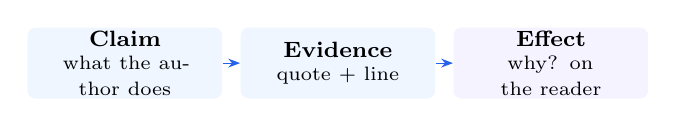
\begin{tikzpicture}[x=1mm,y=1mm,font=\footnotesize,
  stufe/.style={rounded corners=1mm,fill=primtint,minimum height=9mm,text width=24mm,align=center,inner sep=1pt}]
  \node[stufe] (c) at (0,0) {\textbf{Claim}\\[-0.4mm]{\scriptsize what the author does}};
  \node[stufe,right=2.2mm of c] (e) {\textbf{Evidence}\\[-0.4mm]{\scriptsize quote + line}};
  \node[stufe,right=2.2mm of e,fill=sectint] (f) {\textbf{Effect}\\[-0.4mm]{\scriptsize why? on the reader}};
  \draw[-{Stealth[length=1.5mm]},prim] (c) -- (e); \draw[-{Stealth[length=1.5mm]},prim] (e) -- (f);
\end{tikzpicture}\par\vspace{0.6mm}
\textbf{Conclusion:} sum up how style supports the message.
\end{minipage}

\vspace{1mm}
\textcolor{muted}{\footnotesize Our model paragraph (Baxter: respect for Helsinki's achievements) — mark \textbf{C}, \textbf{E}, \textbf{E}:}
\lsglinien{5}{(C) Baxter expresses respect for Helsinki's achievements through appreciative vocabulary. (E) Although she admits that the gig lacked “the buzz of being at a ‘proper’ concert” (ll.\,11–12), she stresses that “technically, it was impressive” (ll.\,12–13) and praises a “world of meticulously rendered make-believe” (ll.\,14–15). (E) Because she first concedes a weakness, her praise sounds balanced and credible, so readers are more likely to share her positive view of the city's innovation.}

\vspace{1mm}
\kl{2d\enspace Evaluation answers (III)}\enspace{\small take a clear position \pfeil arguments with examples (also from the text) \pfeil consider the other side \pfeil justified conclusion. Keep your opinion separate from the facts.}
\end{wsbox}

% ================================================================== Seite 2
\newpage
% ------------------------------------------------------------------ 3
\begin{wsbox}{3}{Step 3 · Editing and checking}
\begin{minipage}[t]{0.485\linewidth}\vspace{0pt}
\kl{Content}\par\vspace{0.3mm}
\begin{itemize}[label=$\square$]
\item I did exactly what the operator asks — no more, no less.
\item Every statement is backed by a line reference.
\item Quotes are marked “…” and exact; omissions as […].
\item I separate facts from my interpretation.
\item My opinion appears only where asked (III).
\end{itemize}
\end{minipage}\hfill
\begin{minipage}[t]{0.485\linewidth}\vspace{0pt}
\kl{Language}\par\vspace{0.3mm}
\begin{itemize}[label=$\square$]
\item present tense to describe the text
\item no contractions (\emph{does not}, not \emph{doesn't}), no \emph{I think} in I/II
\item linking words show my line of thought
\item precise verbs and adjectives instead of \emph{says, good, bad, a lot}
\item no repetition — I varied words and sentence starts
\end{itemize}
\end{minipage}
\end{wsbox}

% ------------------------------------------------------------------ Phrases
\begin{wsbox}{4}{Useful phrases}
\begin{minipage}[t]{0.485\linewidth}\vspace{0pt}
\kl{Giving information on the text}\par
The (article) was written by … and published (online) in (source) on (date). · It deals with / provides insight into …\par\vspace{0.8mm}
\kl{Talking about the structure}\par
In the first paragraph, the author presents … · In the next section, the reader's attention is drawn to … · The following paragraphs provide more details on / examples of … · The author's line of argumentation starts off with … and culminates in …\par\vspace{0.8mm}
\kl{Reporting verbs (instead of \emph{says})}\par
states · claims · argues · points out · explains · emphasises · stresses · criticises · warns · suggests · concedes · admits · concludes
\end{minipage}\hfill
\begin{minipage}[t]{0.485\linewidth}\vspace{0pt}
\kl{Talking about language and style}\par
The author strictly separates / often mixes fact and opinion. · The repetition of … / The use of words such as … emphasises / underlines … · The detailed description of … evokes … / makes the reader feel …\par\vspace{0.8mm}
\kl{Describing tone and register}\par
neutral · matter-of-fact · objective / subjective · formal / informal / colloquial · enthusiastic · appreciative · sceptical · critical · ironic · humorous · emotive · alarming · urgent · optimistic\par\vspace{0.8mm}
\kl{Summing up}\par
All in all, the author gives an unbiased / a rather biased account of … · The text presents the facts in a clear and objective / a very subjective way. · This enables the reader to draw their own conclusions.
\end{minipage}
\end{wsbox}

% ------------------------------------------------------------------ Linking + Quoting
\begin{wsbox}{5}{Linking words and quoting}
\begin{minipage}[t]{0.485\linewidth}\vspace{0pt}
\renewcommand{\arraystretch}{1.1}
\begin{tabularx}{\linewidth}{@{}p{17mm}X@{}}
\textbf{adding} & furthermore, moreover, in addition, apart from that\\
\textbf{contrast} & however, nevertheless, in contrast, whereas, while\\
\textbf{cause/effect} & therefore, thus, consequently, as a result, since\\
\textbf{example} & for instance, to illustrate this, as shown by\\
\textbf{order} & first of all, subsequently, finally\\
\textbf{concluding} & all in all, to sum up, on the whole\\
\end{tabularx}
\end{minipage}\hfill
\begin{minipage}[t]{0.485\linewidth}\vspace{0pt}
\begin{itemize}
\item \textbf{Integrate} quotes into your sentence: Baxter calls the platform a “digital twin” (l.\,16).
\item \textbf{Line references:} (l.\,5) · (ll.\,5–7) · (ll.\,5\,f.) \enspace paraphrase: (cf.\ l.\,5)
\item \textbf{Omissions} […]; \textbf{changes} in square brackets [ ].
\item Never let a quote stand alone — always \textbf{explain} it.
\end{itemize}
\end{minipage}
\end{wsbox}

% ------------------------------------------------------------------ Devices
\begin{wsbox}{6}{Stylistic devices you meet in factual texts — and what they can do}
\renewcommand{\arraystretch}{1.12}
\begin{tabularx}{\linewidth}{@{}>{\raggedright\arraybackslash}p{38mm}>{\raggedright\arraybackslash}X>{\raggedright\arraybackslash}p{38mm}>{\raggedright\arraybackslash}X@{}}
\kl{Device} & \kl{Typical effect} & \kl{Device} & \kl{Typical effect}\\\arrayrulecolor{rule}\midrule
personal anecdote, first person & makes the topic concrete and relatable & expert quotes, statistics & add authority and credibility\\
rhetorical question & involves the reader, guides the argument & contrast / antithesis & highlights differences, sharpens a point\\
enumeration, rule of three & stresses scope, sounds complete and memorable & repetition, anaphora & emphasises a key idea, creates rhythm\\
metaphor, comparison & makes abstract ideas vivid & hyperbole, emotive language & arouses feelings, creates urgency\\
direct address, inclusive \emph{we} & creates closeness, shared responsibility & colloquial words & informal, light tone; reaches a wide audience\\
short sentence after long ones & creates emphasis, a punchline & irony & criticises indirectly, entertains\\
\end{tabularx}\par\vspace{0.6mm}
{\footnotesize Name the device \emph{and} its function in \emph{this} text — a list of devices without effect earns little.}
\end{wsbox}

\vspace{1mm}
\begin{secbox}
\klsec{Online:} the step-by-step course, fold-out tips and the writing coach for your own answers:\enspace \textbf{edu-mrh.de \pfeil Englisch \pfeil Klasse 13 \pfeil Questions on the Text}
\end{secbox}

\end{document}
